\documentclass[conference]{IEEEtran}
%\IEEEoverridecommandlockouts
% The preceding line is only needed to identify funding in the first footnote. If that is unneeded, please comment it out.
\usepackage{cite}
\usepackage{amsmath,amssymb,amsfonts}
\usepackage{algorithmic}
\usepackage{graphicx}
\usepackage{textcomp}
\usepackage{xcolor}
\usepackage{graphicx}
\usepackage{caption}
\usepackage{subcaption}
\usepackage{hyperref}
\def\BibTeX{{\rm B\kern-.05em{\sc i\kern-.025em b}\kern-.08em
    T\kern-.1667em\lower.7ex\hbox{E}\kern-.125emX}}
\begin{document}

\title{TwinViewCV: A Unity-Based Pipeline for Multi-View Dataset Generation and 3D Reconstruction Evaluation\\}


\author{\IEEEauthorblockN{Valeria Itrat Herrera}
\IEEEauthorblockA{\textit{Department of Electrical and Computer Engineering} \\
\textit{Rice University}\\
Houston, TX, USA \\
vi6@rice.edu}
}


\maketitle

\begin{abstract}
Recent advances in 3D reconstruction methods, such as Gaussian Splatting, have demonstrated impressive visual quality from multi-view imagery. However, evaluating and comparing these methods remains challenging due to the limited availability of datasets with controlled camera configurations and reliable ground truth. Most existing datasets rely on fixed real-world camera setups, making systematic ablation studies and reproducibility difficult.
This project proposes a Unity-based pipeline for generating synthetic datasets and evaluating 3D reconstruction methods. The pipeline enables parametrized camera rigs, flexible scene configuration,
and scalable data capture under controlled conditions. Generated datasets are used to reconstruct 3D scenes using Gaussian Splatting and evaluated through image-based metrics. In addition, a calibration pipeline based on OpenCV is implemented to estimate intrinsic and extrinsic camera parameters and compare them with the ground-truth parameters available in the simulated environment. Preliminary results show accurate pose recovery.
\end{abstract}

\begin{IEEEkeywords}
Multi-View, Camera rig, Unity Simulation, 3D reconstruction, Gaussian Splatting
\end{IEEEkeywords}

\section{Introduction}
In recent years, significant advances have been made in computer vision; however, most modern approaches require large amounts of data for training and evaluation. For this reason, many research efforts have explored the use of simulation platforms such as Unity and NVIDIA Omniverse to generate synthetic datasets that can support the development, training, and evaluation of computer vision models \cite{unitySynthetic,synthetic}.

Among the areas that have evolved considerably, 3D reconstruction has received particular attention \cite{overview}. Acquiring datasets for 3D reconstruction is especially challenging, since these methods require not only reliable ground truth for evaluation but also multi-view image datasets captured with synchronized cameras arranged in configurations that provide the visual information required by each reconstruction algorithm. Recent efforts, such as those developed by Dolby Laboratories, have demonstrated the potential of simulated environments for generating multi-view datasets \cite{volucapture}.

This work proposes the development of an open-source Unity-based platform that enables users to create customizable, versatile simulated multi-camera environments for the research and evaluation of 3D reconstruction algorithms, such as Gaussian Splatting \cite{3dgs}. To build a reliable and useful simulation framework, this first stage of the project focuses on validating two key aspects: (1) the synchronization of the multi-camera capture pipeline, (2) the accuracy of the simulated camera calibration when compared with the ground-truth parameters available in the Unity environment, and (3) the feasibility of generating datasets that can be used for 3D reconstruction experiments. These steps provide a foundation for later comparison with a real laboratory camera setup.

The implementation of the proposed framework is available at
\href{https://rice-exp-lab.github.io/universal-reconstruction-simulator/}{https://rice-exp-lab.github.io/universal-reconstruction-simulator/}.

% -------------------------------------------------------- %

\section{Methods}

The system is implemented in Unity, allowing flexible configuration of camera rigs, capture parameters, and calibration setups. The platform supports two operational modes. The first mode enables multi-view image capture from simulated cameras to generate datasets for 3D reconstruction algorithms. The second mode enables camera calibration using a ChArUco board and the OpenCV library.

\subsection{Simulated Environment}

The project is developed using the Unity High Definition Render Pipeline (HDRP), which provides advanced rendering capabilities, including physically-based lighting and camera effects.

The simulated environment represents an indoor laboratory scene where a multi-camera system would be deployed in practice (Figure \ref{fig:lab}). The scene includes configurable lighting conditions and camera effects to emulate realistic acquisition scenarios.

A camera rig generation script allows users to automatically create camera arrays around a target object. The user specifies the number of cameras, their heights, radial distances from the object, and angular distribution. The cameras are then placed evenly around the object to simulate typical multi-view capture configurations.

\begin{figure}[ht] 
\centering 
\begin{subfigure}[b]{0.3\textwidth} 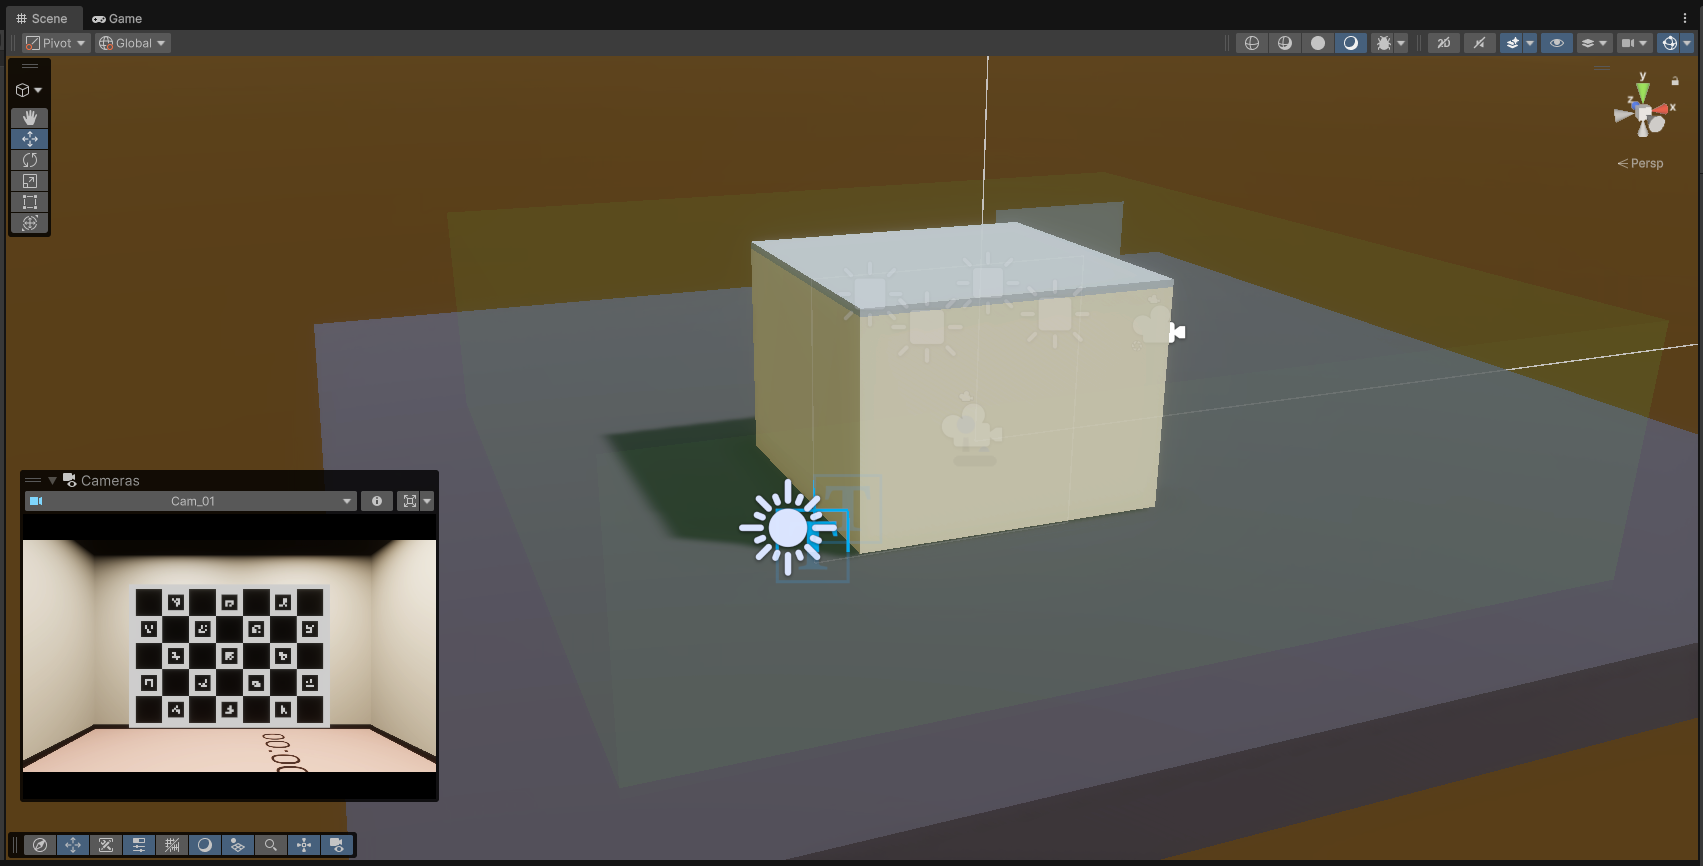
\includegraphics[width=\textwidth]{images/lab_out.png} \caption{Lab building} 
\end{subfigure} 
\hfill 
\begin{subfigure}[b]{0.3\textwidth} 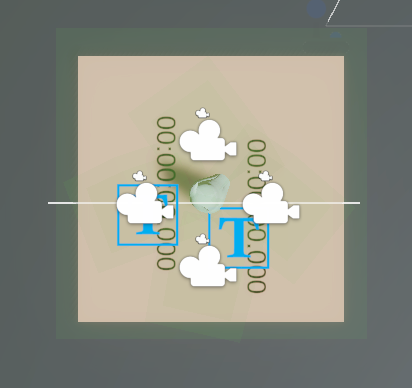
\includegraphics[width=\textwidth]{images/lab_in_top2.png} \caption{Multiple camera setup} 
\end{subfigure} 
\caption{Simulated laboratory environment in Unity.} \label{fig:lab} 
\end{figure}

To increase the variety of viewpoints and capture conditions, camera motion can be introduced during acquisition. The system supports different motion patterns, including linear translation and circular or spiral trajectories around the target object.

\subsection{Camera Modeling}
The simulated cameras are configured using Unity’s Physical Camera model. The camera parameters are based on the specifications of the Orbbec Femto Mega camera, which will be used in the real-world setup.

The camera model includes parameters such as sensor size, focal length, and field of view. Additionally, Unity’s HDRP local volumes support optical effects, such as depth of field and lens distortion, enabling experimentation with different imaging conditions.

\begin{itemize}
    \item Sensor size: $5.568 \times 3.84$
    \item Focal length: $3.317$
    \item Horizontal field of view: $80^\circ$
    \item Aperture: $f/2.7$
\end{itemize}


\subsection{Dataset Generation}
The platform allows users to generate synthetic datasets by capturing frames from the simulated cameras.

Capture parameters, such as image resolution, frame rate, and the total number of frames, can be configured by the user prior to acquisition. To verify the timing accuracy of the capture process and ensure proper synchronization when multiple cameras are used, a digital timer object that displays timestamps with millisecond precision is placed in the scene and recorded in the captured frames.

\subsection{3D Gaussian Splatting Reconstruction}

For the reconstruction experiments, the official implementation of 3D Gaussian Splatting provided by INRIA was used \cite{gaussian-splatting}.

The dataset was generated by moving the camera along a spiral trajectory around a static object. The capture was performed at 15 frames per second over a 15-second interval, resulting in a dataset of 225 images.

 The overall workflow of the dataset generation and reconstruction process is shown in Figure \ref{fig:pipeline}.

 \begin{figure}[htbp]
    \centering
    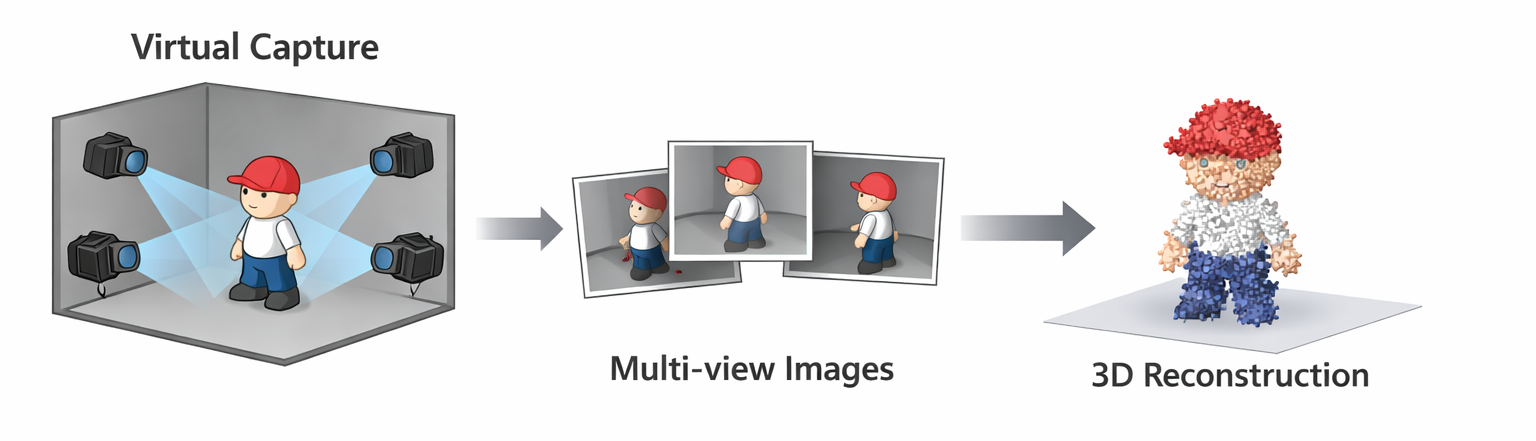
\includegraphics[width=\linewidth]{images/multi_view.png}
    \caption{Multi-view dataset application pipeline}
    \label{fig:pipeline}
\end{figure}

Two capture configurations were tested. In the first experiment, the camera completed three full rotations around the object during the capture interval. In the second configuration, the camera performed two rotations over the same duration, resulting in a slower camera motion and improved view coverage.

The second configuration produced a significantly better reconstruction, while the first failed to recover the full geometry of the object.

\subsection{Camera Calibration}
To estimate the intrinsic and extrinsic parameters of the simulated camera, a calibration pipeline based on OpenCV for Unity was implemented \cite{openCV}.

A ChArUco calibration board is generated in the Unity scene using configurable parameters, including the number and size of squares, the marker size, and the dictionary type.

During calibration mode, markers and board corners are detected in the captured frames using OpenCV’s ArUco detection algorithms and displayed in the preview view. 
The user captures multiple frames as they move the board to different positions and orientations to obtain a diverse set of observations. Once a sufficient number of frames have been collected, the calibration procedure is executed to estimate the intrinsic camera matrix and the extrinsic parameters relative to the calibration board.


These estimated parameters are later be compared with the ground-truth camera parameters available from the Unity simulation. 

The calibration pipeline implemented in the system is illustrated in Figure \ref{fig:calibration}.

 \begin{figure}[htbp]
    \centering
    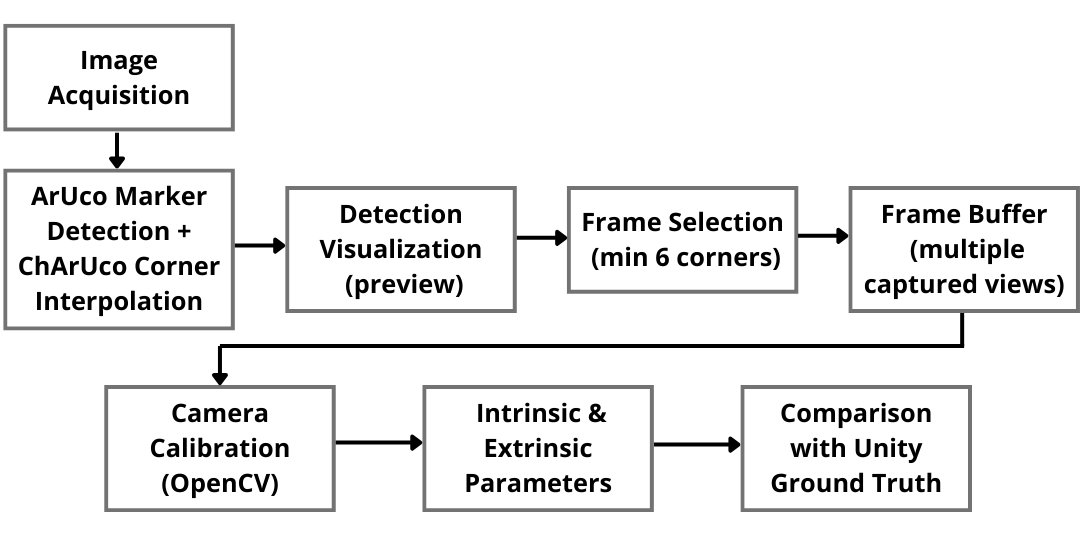
\includegraphics[width=\linewidth]{images/calibration.png}
    \caption{Calibration pipeline}
    \label{fig:calibration}
\end{figure}

% -------------------------------------------------------- %
\section{Results}

\subsection{Dataset}

To evaluate the synchronization of the camera rig when working with multiple cameras, four cameras were placed around the target object in the scene, each following different motion trajectories at 15 FPS. Frames captured by different cameras at the same time step share matching timestamps, and the corresponding entries in the dataset metadata reflect the same acquisition time.

To further verify the synchronization of the capture process, a digital clock displaying time with millisecond precision was placed on the floor of the scene. The clock is visible from all camera views, allowing direct visual confirmation that frames captured at the same timestep correspond to the same timestamp across the different cameras.

This confirms that the capture pipeline maintains correct synchronization across the camera rig.


\subsection{3D Gaussian Splatting Reconstruction}

The reconstruction results obtained using the generated dataset are promising. The quantitative metrics calculated on the training dataset are shown in Table~\ref{tab:results}. These results indicate that the model successfully converged and that the reconstruction provides a good approximation of the scene geometry and appearance (Figure \ref{fig:3dgs}). 

 \begin{figure}[htbp]
    \centering
    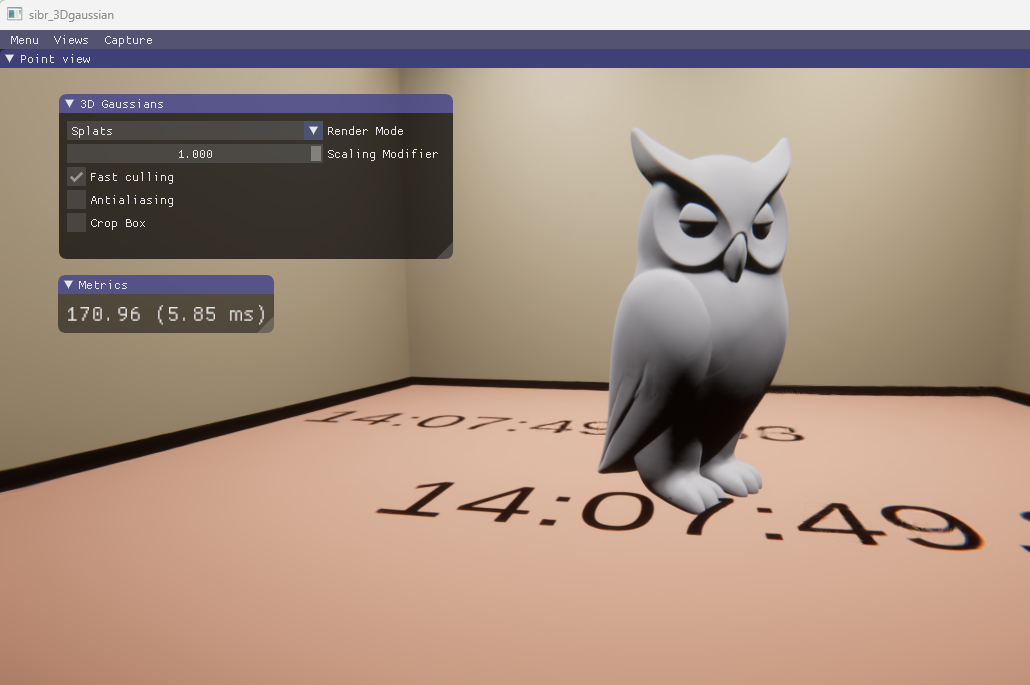
\includegraphics[width=\linewidth]{images/3dgs.png}
    \caption{Reconstructed scene using Gaussian Splatting.}
    \label{fig:3dgs}
\end{figure}

A visualization of the reconstruction can be seen in the video available at \href{https://youtu.be/-RY_b5SnkdY}{https://youtu.be/-RY\_b5SnkdY}.


\begin{table}[!t]
  \centering
  \begin{tabular}{lc}
    \hline
    Metric & Result \\
    \hline
    PSNR & 30.99 dB \\
    SSIM & 0.986 \\
    LPIPS & 0.029 \\
    \hline
  \end{tabular}
  \caption{3DGS reconstruction metrics.}
  \label{tab:results}
\end{table}

\subsection{Camera Calibration}

%The intrinsic camera matrix estimated using the OpenCV calibration pipeline is

%\begin{equation}
%K =
%\begin{bmatrix}
%761.65 & 0 & 639.87 \\
%0 & 761.67 & 359.50 \\
%0 & 0 & 1
%\end{bmatrix}
%\end{equation}

The reprojection root mean square (RMS) error of the calibration is 0.153 pixels. The focal length values $(f_x, f_y)$ are nearly identical, which is consistent with the expected behavior of the camera model. In addition, the estimated principal point $(c_x, c_y)$ is close to the center of the image resolution (1280×720), indicating that the intrinsic parameters are consistent with the simulated camera configuration.

%The rotation matrix estimated by OpenCV is

%\begin{equation}
%R =
%\begin{bmatrix}
%0.99224 & 0.12435 & -1.74\times10^{-5} \\
%-0.12343 & 0.98488 & -0.12157 \\
%-0.01510 & 0.12063 & 0.99258
%\end{bmatrix}
%\end{equation}

The estimated rotation was compared with the ground-truth rotation obtained from Unity. The angular difference between the two rotations was approximately $0.0000^\circ$, indicating near-perfect alignment between the estimated pose and the simulated ground truth.

%The translation vector estimated by the OpenCV calibration is

%\begin{equation}
%t =
%\begin{bmatrix}
%-0.343 \\
%-0.196 \\
%0.628
%\end{bmatrix}
%\end{equation}

The translation error between the estimated pose and the Unity ground truth is approximately 1.0 mm.

%\begin{table}[h]
%\centering
%\begin{tabular}{lcc}
%\hline
%Parameter & Error \\
%\hline
%Rotation error & \multicolumn{2}{c}{0.0000°} \\
%Translation error & \multicolumn{2}{c}{1.00 mm} \\
%Re-projection error (RMS) & \multicolumn{2}{c}{0.153} \\
%\hline
%\end{tabular}
%\caption{Comparison between OpenCV calibration and Unity ground-truth.}
%\label{tab:resultsCalib}
%\end{table}

%The results in Table \ref{tab:resultsCalib} 
These results indicate that the calibration pipeline implemented in the simulated environment accurately recovers the camera pose relative to the ChArUco board, achieving millimeter translation accuracy and negligible rotation error.

\section{Discussion}  

The preliminary results obtained in this work are promising and suggest that the simulated environment can serve as a feasible benchmark for generating synthetic datasets for 3D reconstruction experiments. The platform provides flexibility for configuring synchronized multi-view camera setups and generating controlled acquisition conditions.

The calibration pipeline using a single camera was successfully implemented and validated by comparing the parameters estimated with OpenCV against the ground-truth camera parameters available from the Unity simulation.

However, further work is required to evaluate how closely the simulated calibration results match those obtained from a real camera setup. Future work will focus on extending the calibration procedure to multi-camera configurations and on performing laboratory experiments using the same camera arrangement as in the simulated environment. These experiments will allow a direct comparison between simulated and real results.

\section*{Acknowledgment}
The authors declare no potential conflicts of interest.

The author thanks Prof. Robert LiKamWa and Krutik Pandya for their guidance and support throughout this project.

\section*{CRediT Author Statement}
Valeria Itrat Herrera: Conceptualization, Methodology, Software, Investigation, Data Curation, Writing - Original Draft, Writing - Review and Editing

\bibliographystyle{IEEEtran}
\bibliography{references}

\end{document}
